\appendix

%%%%%%%%%%%%%%%%%%%%%%%%%%%%%%%%%%%%%%%%%%%%%%%%%%%%%%%%%%%%%%%%%%%%%%%%%%%%%%%%%%%%%%%%%%%%%%%%%
%
%
%
%%%%%%%%%%%%%%%%%%%%%%%%%%%%%%%%%%%%%%%%%%%%%%%%%%%%%%%%%%%%%%%%%%%%%%%%%%%%%%%%%%%%%%%%%%%%%%%%%
\clearpage
\onecolumngrid
\section{Supplementary Figures}
\setcounter{figure}{0}
\renewcommand{\thefigure}{SF\arabic{figure}}



% --------------- Dim red time series and free energy profiles
\begin{figure}[h!]
    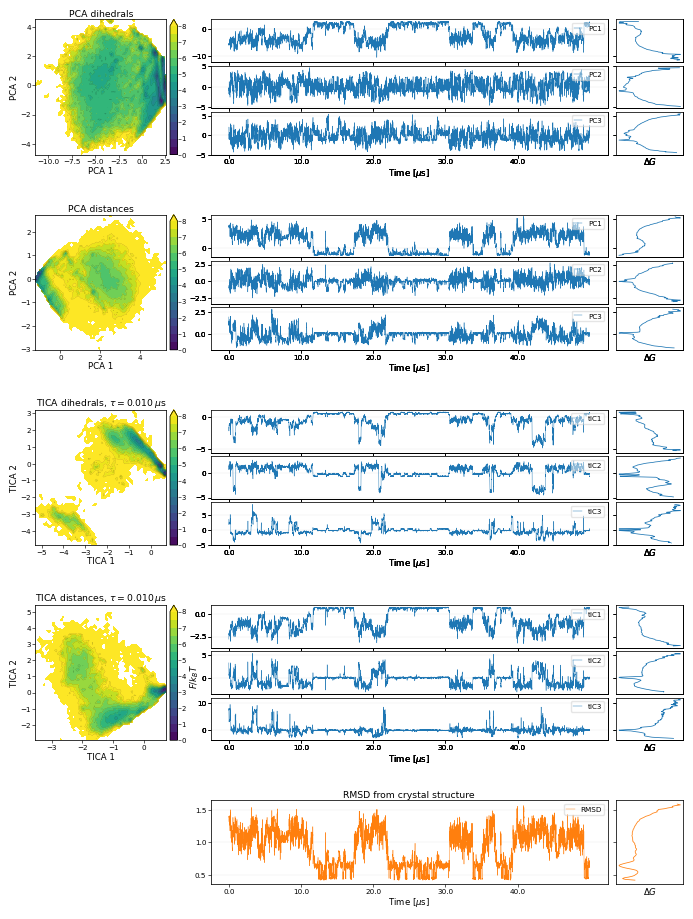
\includegraphics[width=0.8\linewidth]{figures/RMSD_reduced_projection_A4.png}
\caption{\small
Comparison of the compressed trajectory representations obtained from the four feature--dimensionality-reduction pipelines. 
Rows correspond to PCA dihedrals, PCA contact distances, TICA dihedrals, and TICA contact distances. 
The left column shows the projection onto the first two reduced coordinates. 
The right block shows, for each pipeline, the time series of the first three reduced coordinates over the first $40\,\mu\mathrm{s}$, together with the corresponding one-dimensional free-energy profiles computed from the full trajectory. 
The bottom row reports the RMSD from the crystal structure and its one-dimensional free-energy profile as a reference folding coordinate. 
The PCA projections show mostly unimodal one-dimensional free-energy profiles and less pronounced residence-and-jump behavior with respect to the tICA representations. 
}
    \label{suppfig:dimred_figure}
\end{figure}


% --------------- MSM connectivity and active population as a function of lag time
\begin{figure}[h!]
    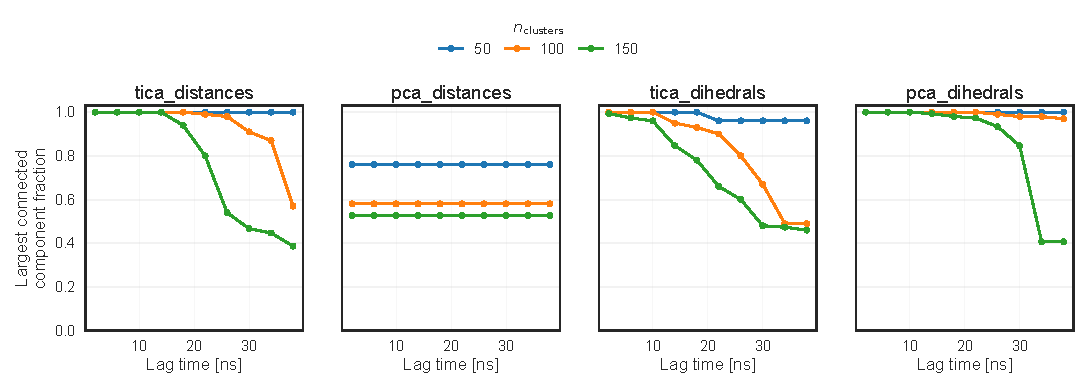
\includegraphics[width=0.7\linewidth]{figures/largest_connected_component_vs_lag.pdf}
    
\includegraphics[width=0.7\linewidth]{figures/active_population_vs_lag.pdf}
    \caption{\small \textbf{MSM connectivity and active population as a function of lag time.}
    Top panel: fraction of microstates in the largest connected component of the MSM as a function of lag time. 
    Bottom panel: fraction of the total equilibrium population contained in the largest connected component of the MSM as a function of lag time}
    \label{suppfig:largest_connected_component_vs_lag}
\end{figure}


% -------------- CK test

\begin{figure}[h!]
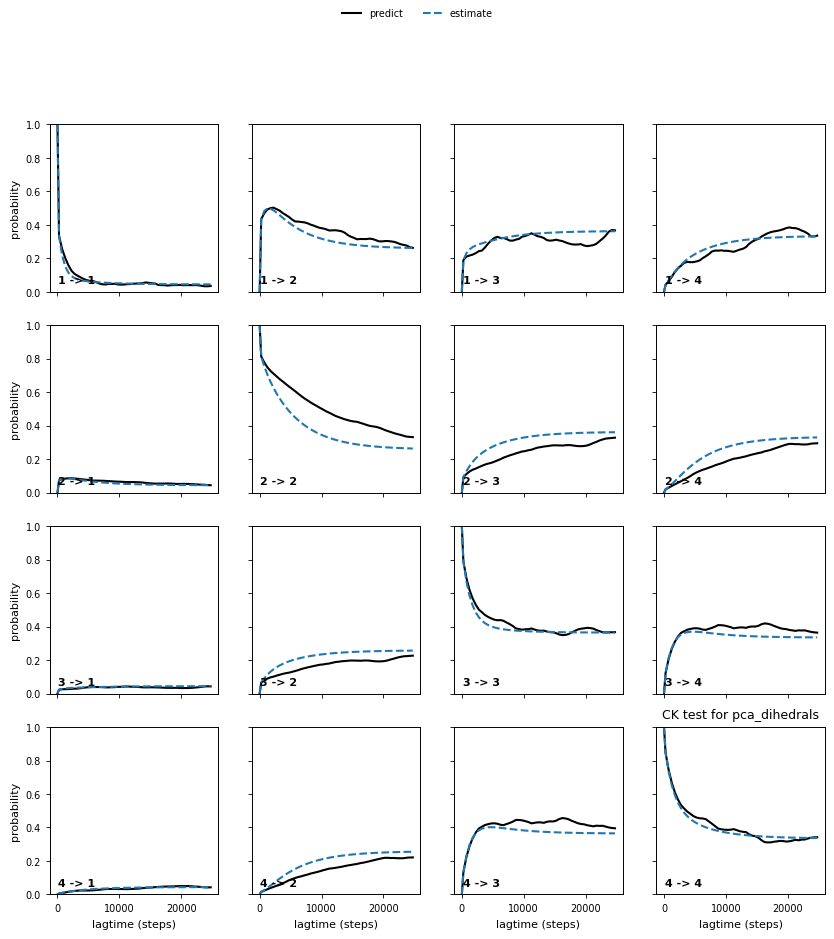
\includegraphics[width=0.7\linewidth]{figures/CK_example.png}
\caption{Chapman--Kolmogorov test for the pca-dihedrals MSM. The microstate
model estimated at $\tau = 50$\,ns was lumped into four metastable sets with
PCCA++. Each panel ($i\!\to\!j$) shows the probability of being in set $j$ at
time $k\tau$ given the system started in set $i$. Solid lines: MSMs estimated
independently at each lag; dashed lines: predictions from the $\tau = 50$\,ns
model. Close agreement indicates approximate Markovianity at the chosen lag.}
\label{suppfig:ck}
\end{figure}

% ------------- First eigenvector of all models -------------------------
\begin{figure}[!t]
    \centering
    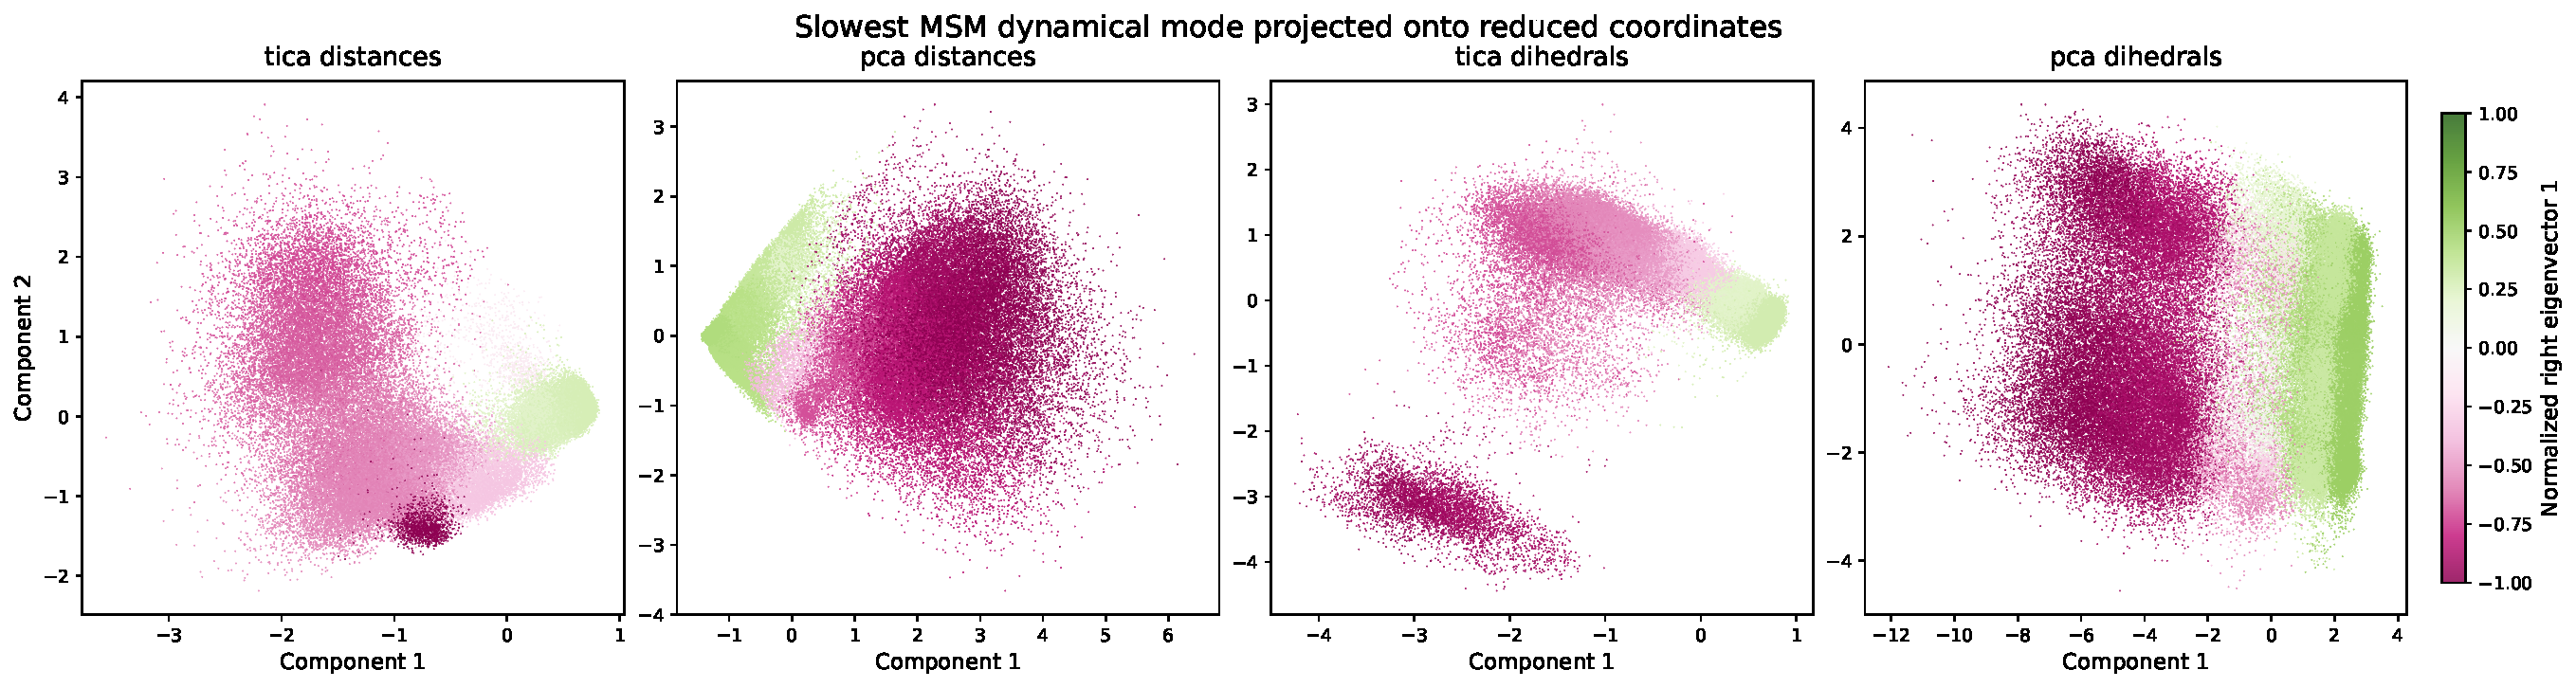
\includegraphics[width=0.8\linewidth]{figures/msm_right_eigenvector_1_projection.pdf}
    \vspace{1em}
    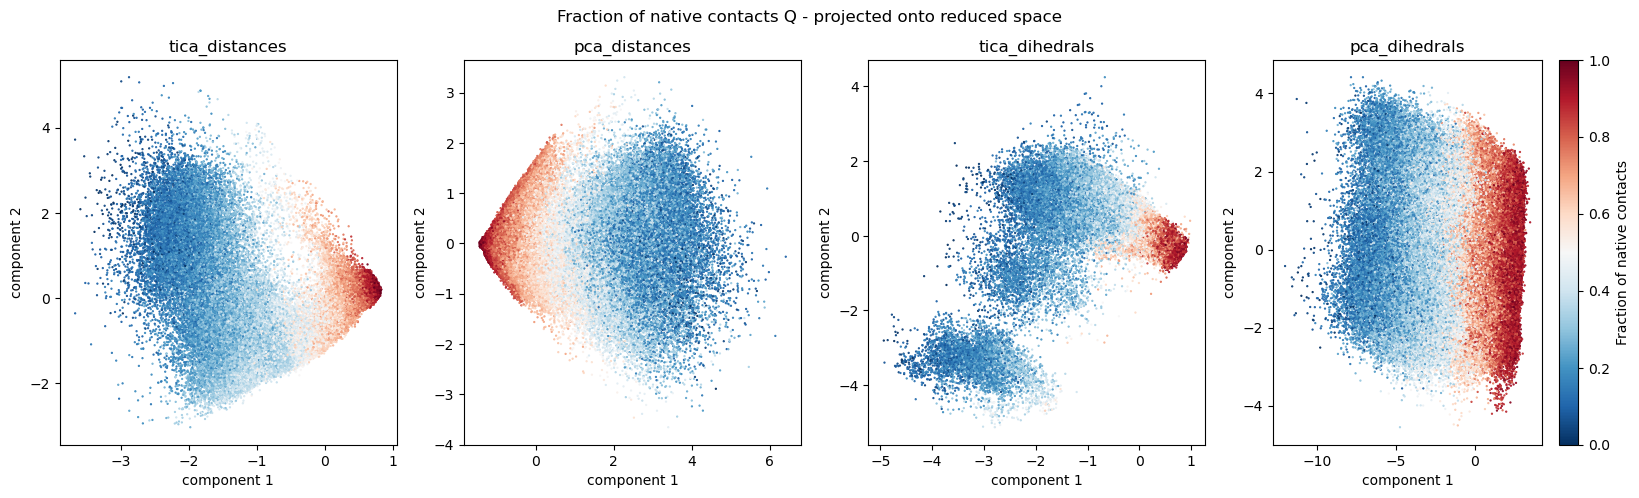
\includegraphics[width=0.8\linewidth]{figures/Q_reduced_projection.png}
    \caption{\footnotesize \textbf{Comparison between the slowest MSM relaxation mode and a structural folding descriptor.} 
    Top row: values of the first non-trivial eigenvector projected onto the first two components of the reduced coordinate space.
    Positive and negative components identify regions that exchange probability on the slowest resolved timescale of the Markov model. 
    Bottom row: projection of the fraction of native contacts, Q, onto the same coordinates. 
    The close correspondence between the eigenvector sign pattern and the distribution of $Q$ indicates that the slowest kinetic process 
    captured by the MSM is associated with the folding-unfolding transition.}
    \label{suppfig:first_right_eigenvector}
\end{figure}



\begin{figure}[h!]
    \centering
    
\includegraphics[width=0.8\linewidth]{figures/pairwise_pcca_membership_scatter_quadrants_report.pdf}
    \caption{\small \textbf{Fuzzy membership probabilities of the trajectory frames to the two macrostates across models.} Each panel shows the fuzzy membership probability of each frame in the trajectory to macrostate $0$ (denatured basin) and macrostate $1$ (native basin) for a different model. The models based on distances (tica-distances and pca-distances) show very similar distributions, while the tica-dihedrals model exhibits a broader distribution, particularly for frames assigned to the denatured basin. This indicates that the tica-dihedrals model has more uncertainty in assigning frames to the denatured basin.}
    \label{suppfig:fuzzy_memberships_models}
\end{figure}



\begin{figure}[h!]
    \centering
    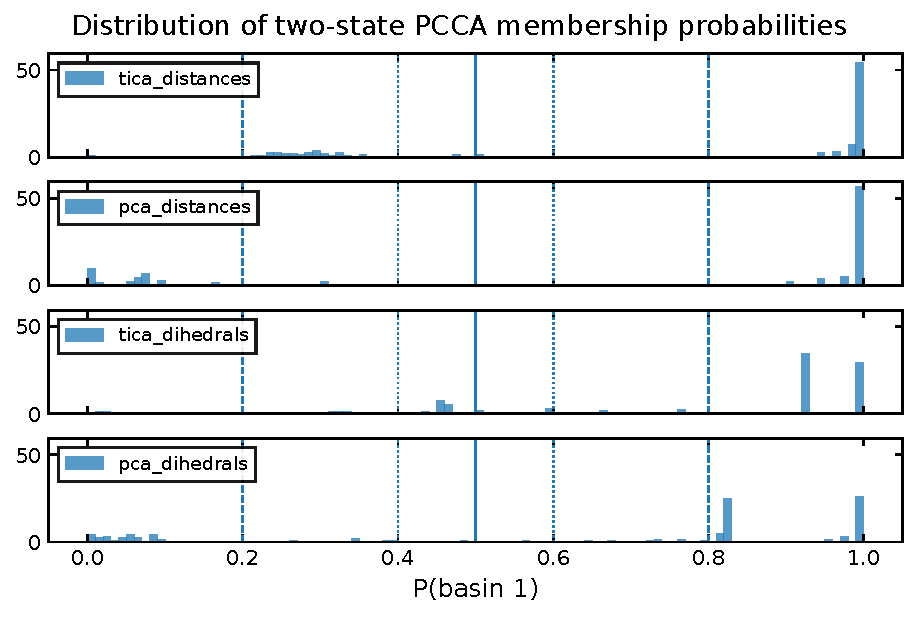
\includegraphics[width=0.8\linewidth]{figures/pcca_membership_probability_distributions.pdf}
    \caption{\small the distributions of fuzzy membership probabilities assigned to frames, for basin $1$ across the four models. }
    \label{suppfig:pcca_frames_prob_density}
\end{figure}


% ------------ Cored  2-state PCCA trajectories -------------------------
\begin{figure}[h!]
    \centering
    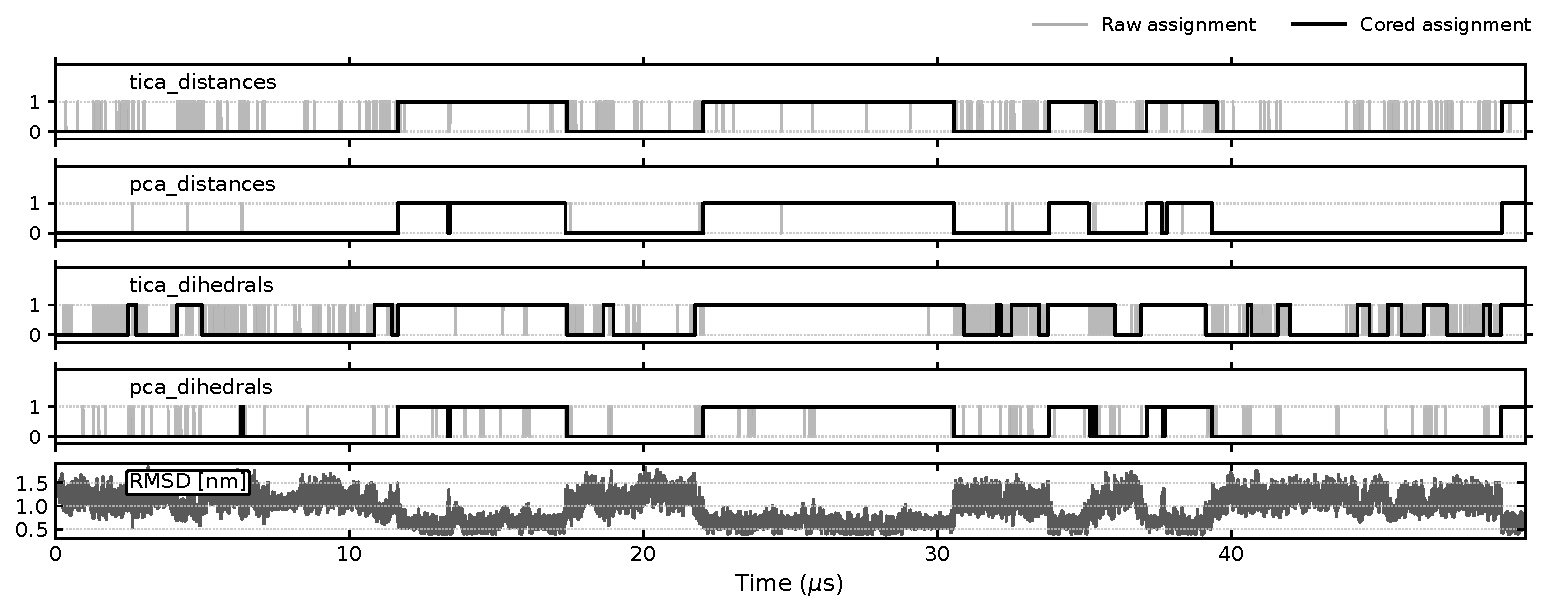
\includegraphics[width=\linewidth]{figures/two_state_raw_vs_cored_assignments.pdf}
    \caption{\small }
    \label{suppfig:twostate_traj}
\end{figure}




% ----- Folded Basin Contact Map and Representative Structures
\begin{figure}[h!]
    \centering
    
\includegraphics[width = 0.8\linewidth]{figures/twostate_helix_differences.pdf}
    \caption{Bottom: overlay of a random sample of $5$ structures from the consensus folded basin. Visualization was made with PyMOL \cite{pymol}.}
    \label{suppfig:twostate_helix}
\end{figure}


% ------ Top ten contacts distinguishing folded basin
\begin{table}
\caption{Top ten residue contacts ranked by the cutoff-free robust folded-contact score. Distances are reported in nm. The robust effect size $d_\mathrm{robust}$ compares the median contact distance outside and inside the folded basin, normalized by the pooled interquartile range. Contact probabilities were computed using a 0.8 nm cutoff and are reported only as auxiliary descriptors.}
\label{tab:top10_folded_contacts}
\begin{tabular}{lccccccc}
\hline
Contact & $\tilde r_\mathrm{folded}$ & $\tilde r_\mathrm{other}$ & $\mathrm{IQR}_\mathrm{folded}$ & $d_\mathrm{robust}$ & $P_\mathrm{folded}$ & $P_\mathrm{other}$ & $\Delta P$ \\
\hline
7--12 & 0.370 & 1.036 & 0.047 & 2.510 & 0.995 & 0.115 & 0.881 \\
9--32 & 0.359 & 1.635 & 0.131 & 2.399 & 0.865 & 0.047 & 0.817 \\
6--17 & 0.422 & 1.381 & 0.101 & 2.219 & 0.973 & 0.092 & 0.881 \\
7--13 & 0.487 & 1.158 & 0.089 & 2.190 & 0.866 & 0.073 & 0.793 \\
6--14 & 0.488 & 1.211 & 0.120 & 2.084 & 0.917 & 0.073 & 0.845 \\
10--32 & 0.529 & 1.602 & 0.209 & 1.825 & 0.665 & 0.059 & 0.606 \\
10--34 & 0.453 & 1.528 & 0.184 & 1.821 & 0.768 & 0.088 & 0.680 \\
10--29 & 0.529 & 1.431 & 0.164 & 1.780 & 0.698 & 0.079 & 0.619 \\
7--11 & 0.317 & 0.712 & 0.053 & 1.776 & 0.996 & 0.349 & 0.647 \\
6--13 & 0.590 & 1.241 & 0.202 & 1.702 & 0.532 & 0.053 & 0.478 \\
\hline
\end{tabular}
\end{table}


% ---------------------------------------------------------
% Survival probability
% ---------------------------------------------------------
\begin{figure}[h!]
    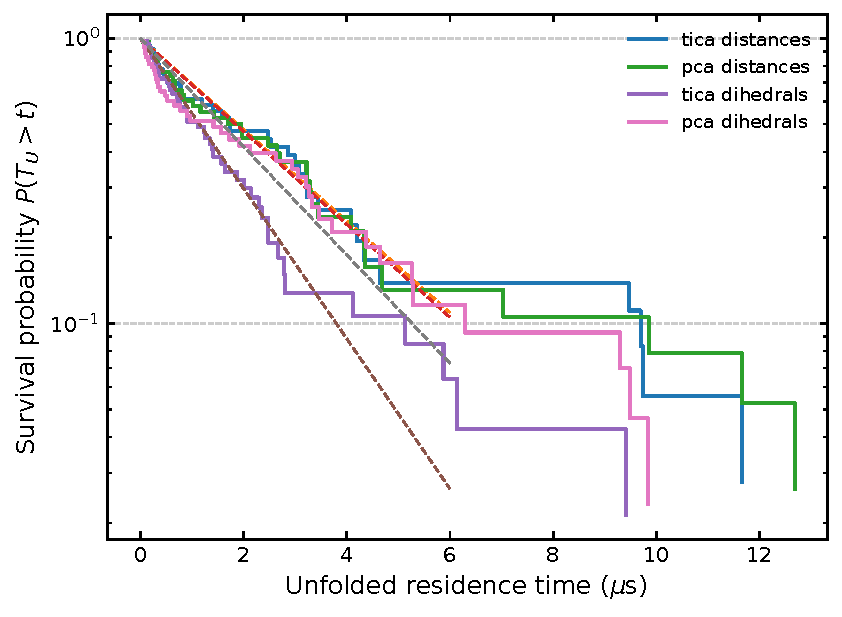
\includegraphics[
        width=0.35\textwidth
    ]{figures/unfolded_residence_times_survival.pdf}
    \caption{Survival probability of the unfolded-state
        residence times.}
    \vspace{0.8em}
\end{figure}



% ---------------------------------------------------------
% Survival probability
% ---------------------------------------------------------
\begin{table}[h!]
    \begin{tabular}{lccccc}
        \hline
        Model
        & $P(S_0)$
        & $P(S_1)$
        & $\langle t_0\rangle$ ($\mu$s)
        & $\langle t_1\rangle$ ($\mu$s)
        & $\Delta G_{1-0}$ (kcal mol$^{-1}$) \\
        \hline
        tICA distances  & 0.230 & 0.770 & 1.591 & 5.312 & -0.863 \\
        PCA distances   & 0.303 & 0.697 & 1.933 & 4.446 & -0.596 \\
        tICA dihedrals  & 0.218 & 0.782 & 1.471 & 5.286 & -0.915 \\
        PCA dihedrals   & 0.358 & 0.642 & 1.407 & 2.520 & -0.417 \\
        \hline
    \end{tabular}
    \caption{Coarse-grained stationary populations and
        mean residence times predicted by the two-state PCCA models. The MSM
        mean residence times were calculated as
        $\langle t_i\rangle=\tau/(1-T_{ii})$, where $\tau$ is the MSM lag
        time. Relative free energies were calculated as
        $\Delta G_{1-0}=-k_{\mathrm B}T
        \ln[P(S_1)/P(S_0)]$ at $T=360$ K.}
    \label{supptab:pcca_model_estimates}
\end{table}

% ------------- Three state tica-distances -------------------------
\begin{figure*}[ht]
    %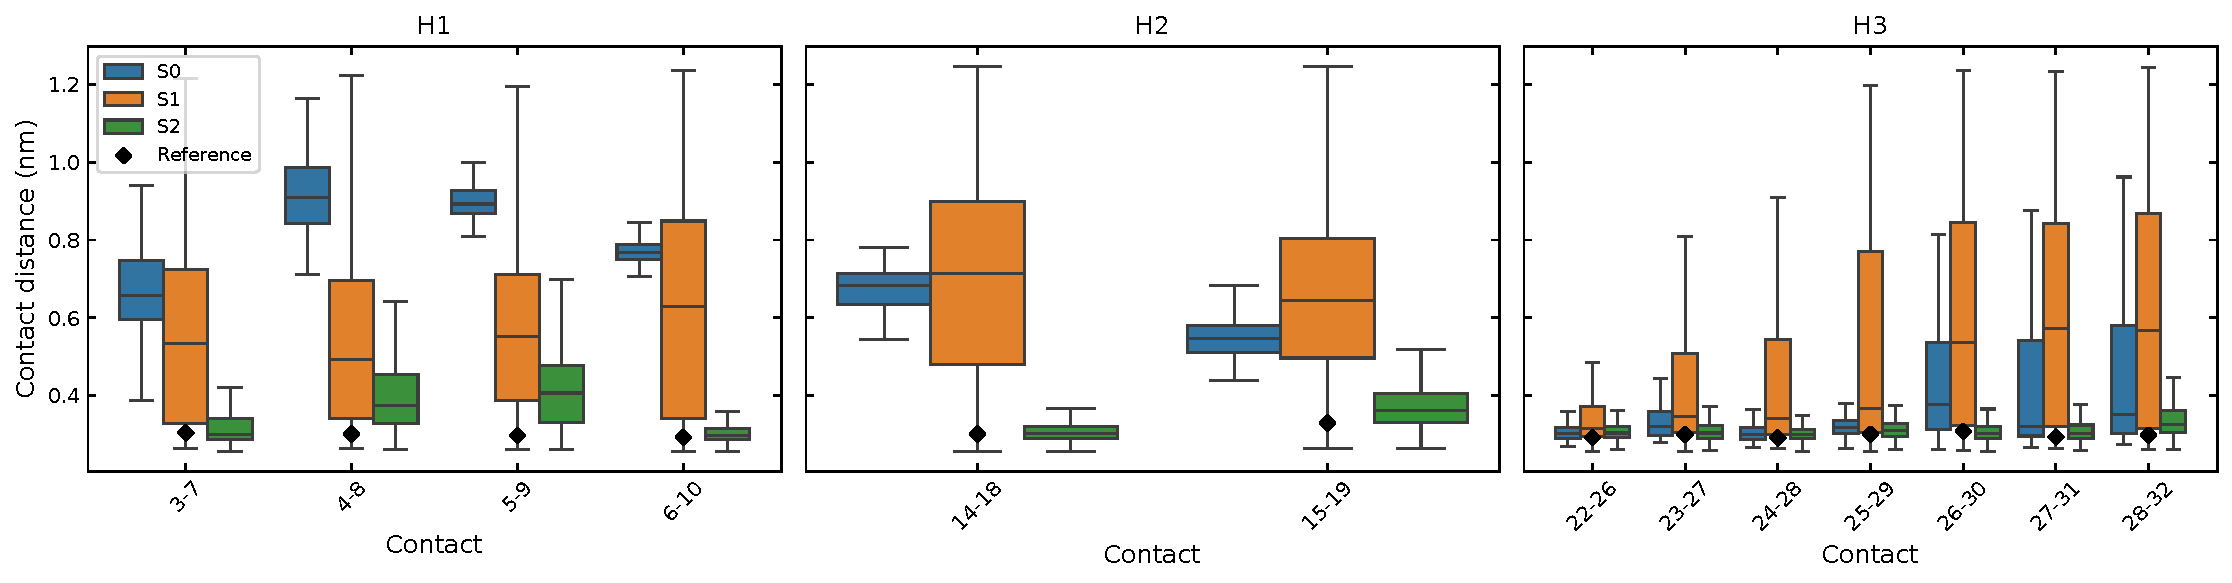
\includegraphics[width=0.7\linewidth]{figures/threestate_tica_helix_differences.pdf}
    %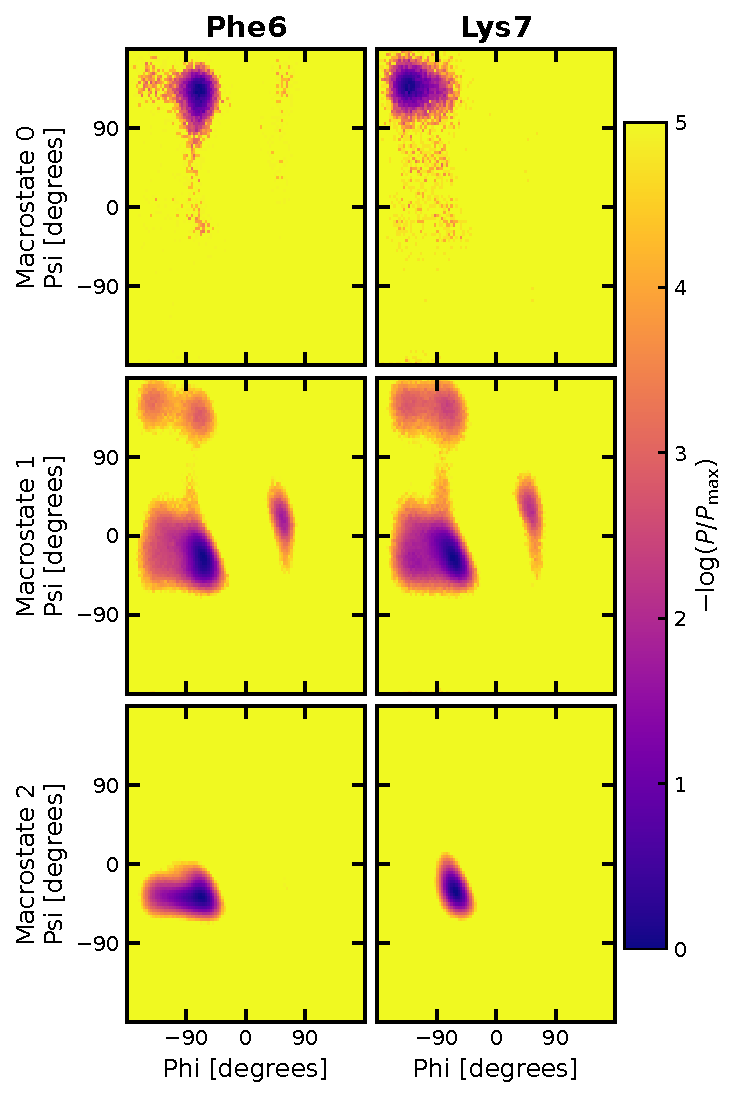
\includegraphics[width=0.2\linewidth]{figures/tica_distances_ramachandran.pdf}
    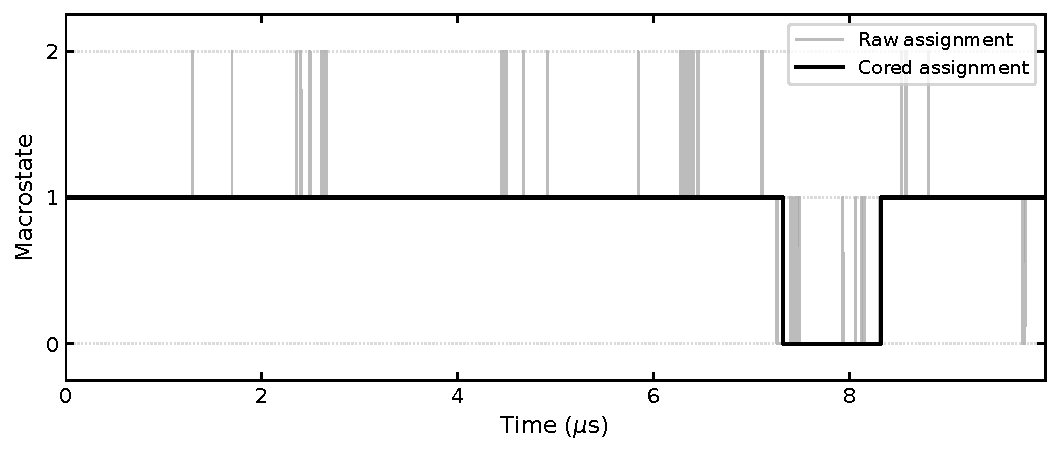
\includegraphics[width=0.7\linewidth]{figures/tica_distances3_pcca_coring_trajectory.pdf}
    \caption{\small {Trajectory of the three-state PCCA++ model for tICA-distances.}}
    \label{suppfig:threestate_distances_traj}
\end{figure*}




% ------------- Three state tica-dihedrals -------------------------
\begin{figure*}[ht]
    %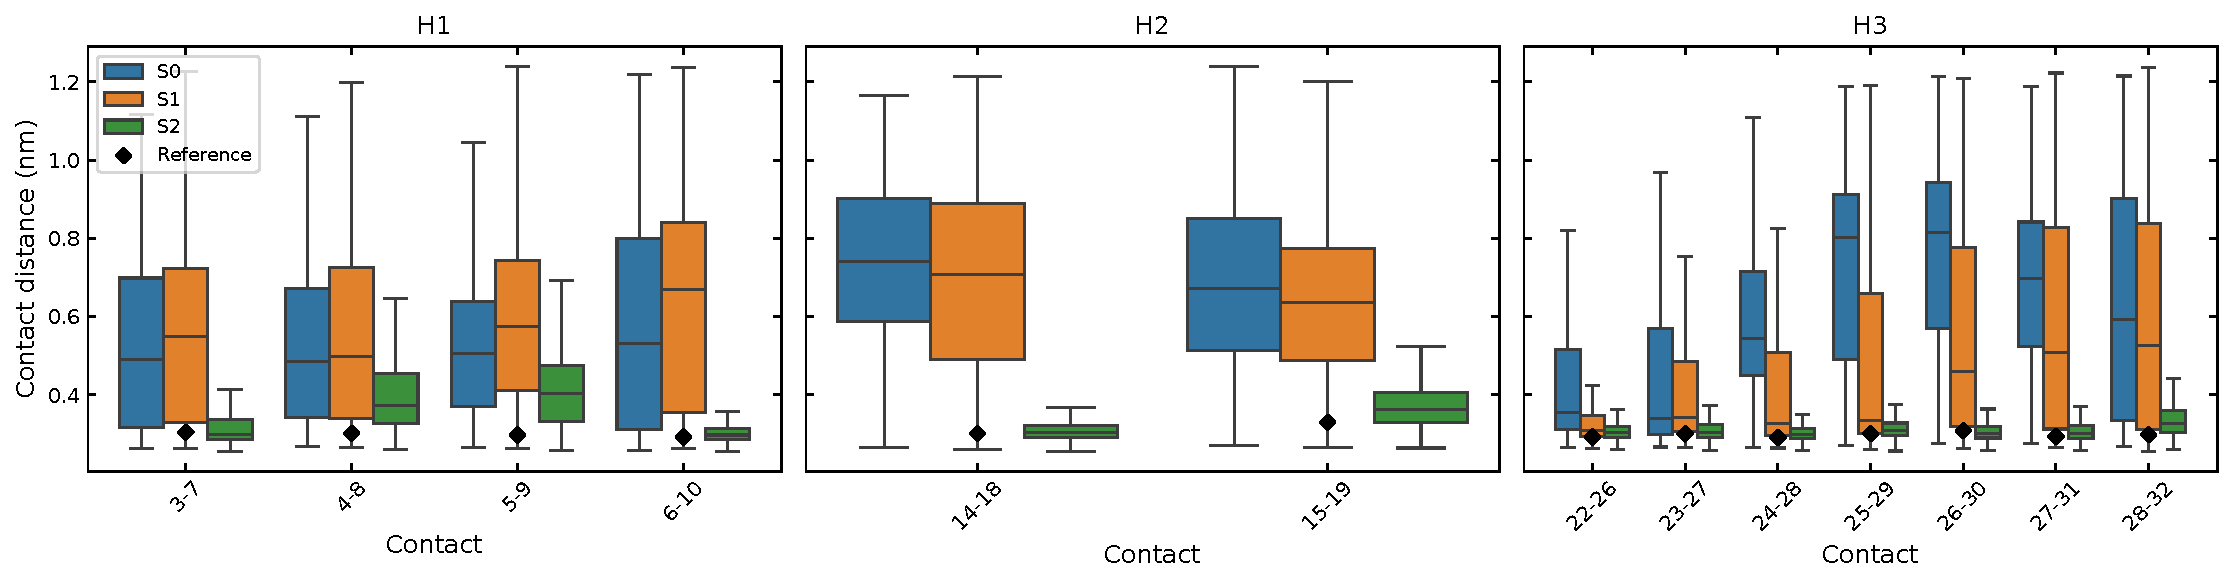
\includegraphics[width=0.7\linewidth]{figures/threestate_dihedrals_helix_differences.pdf}
    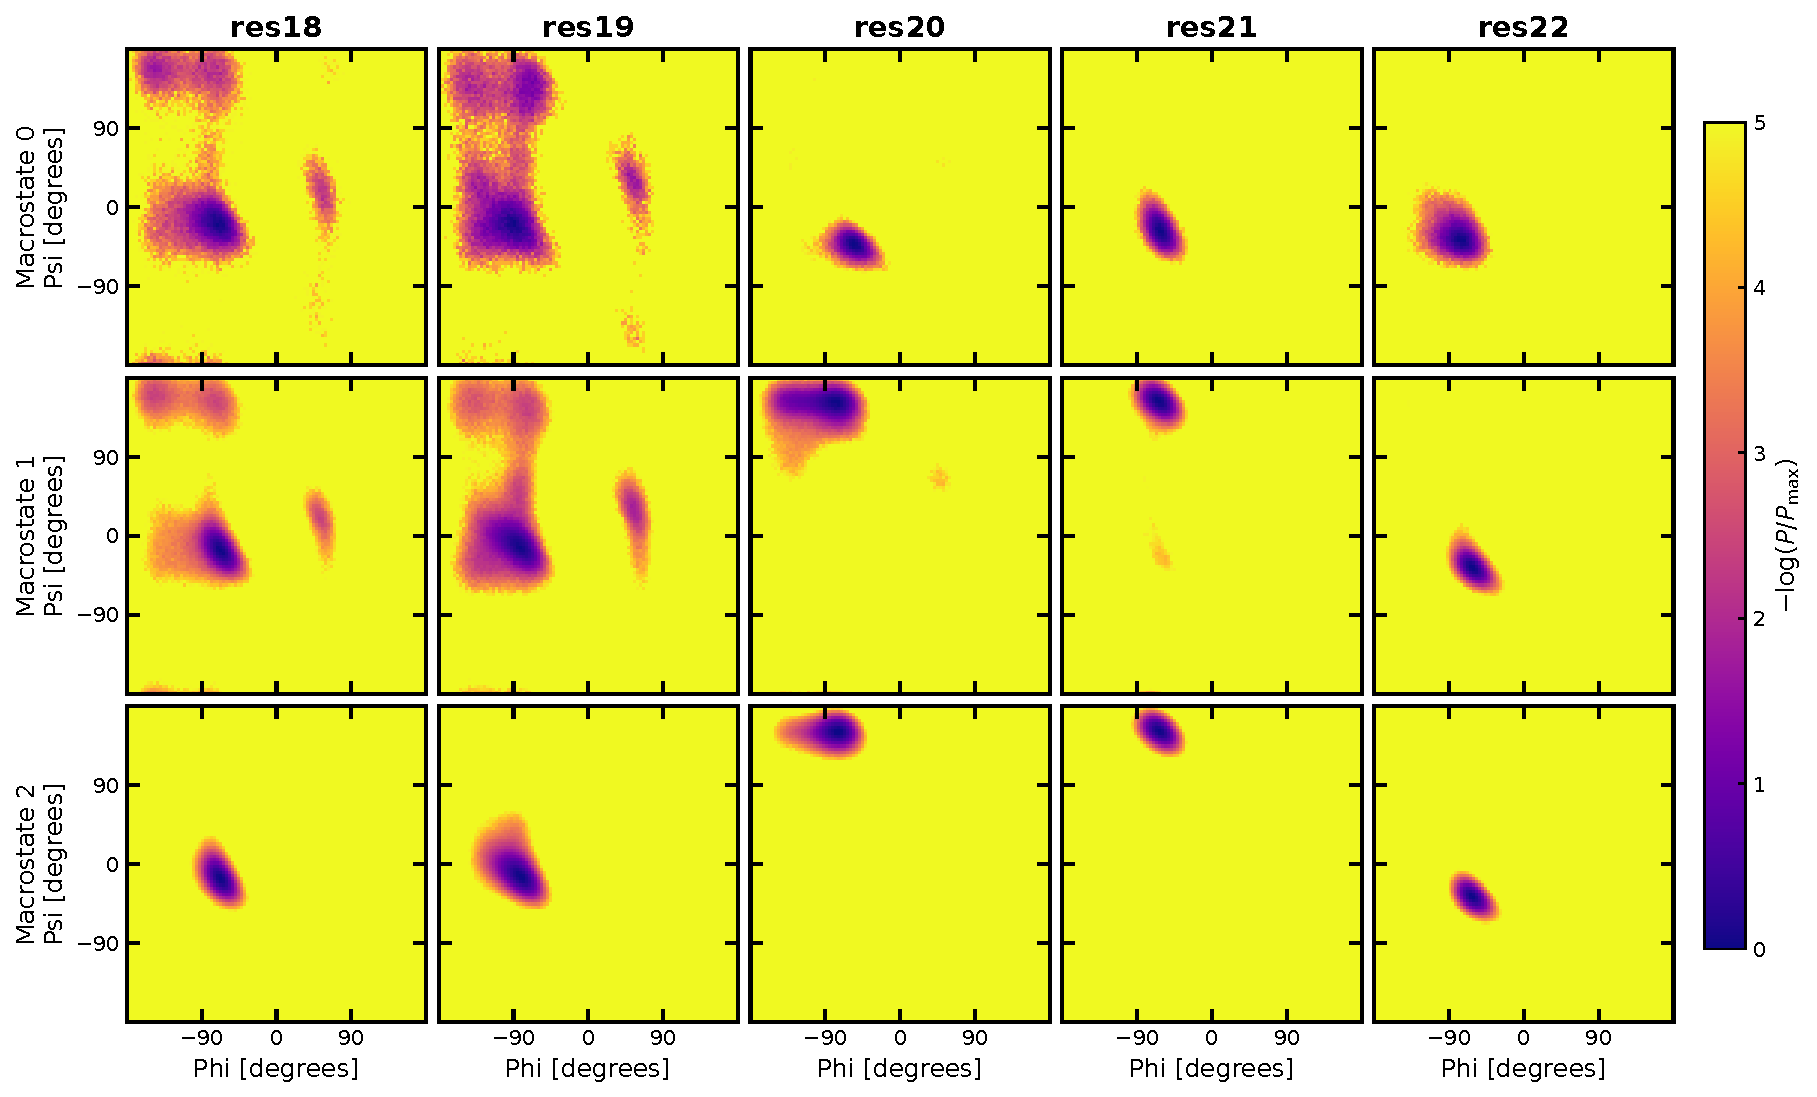
\includegraphics[width=0.8\linewidth]{figures/dihedrals_ramachandran_macrostate_comparison.pdf}
    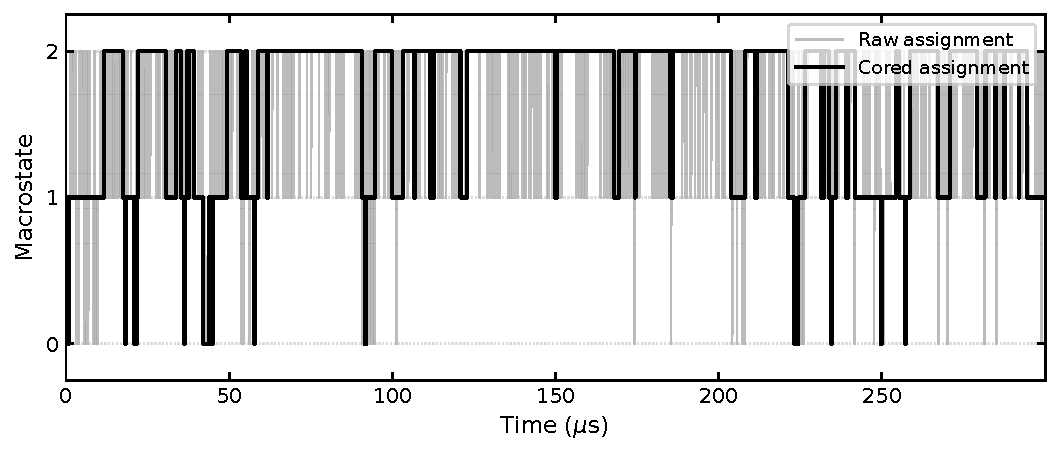
\includegraphics[width=0.8\linewidth]{figures/tica_dihedrals_3_pcca_coring_trajectory.pdf}
    \caption{\small {\textbf{Sturctural caracterization of the 3-state PCCA macrostates for the tica-dihedrals model:} Top: ($\phi, \psi$) distribution of the residues $18-22$ in the three macrostates $S_0, S_1, S_2$.
    Bottom: trajectory of the three-state PCCA++ model for tICA-dihedrals, with hard assignations and cored assignations (transitions are counted if they remain in the destination for at least one markov step, which is $\tau = 50\,ns$).}}
    \label{suppfig:threestate_tica_dihedrals}
\end{figure*}